%\documentclass[10pt,flushrt,preprint]{aastex}

\documentclass[manuscript]{aastex}

\usepackage{graphicx}
\usepackage[space]{grffile}
\usepackage{latexsym}
\usepackage{amsfonts,amsmath,amssymb}
\usepackage{url}
\usepackage[utf8]{inputenc}
\usepackage{fancyref}
\usepackage{hyperref}
\hypersetup{colorlinks=false,pdfborder={0 0 0},}

\usepackage{natbib}

\newcommand{\truncateit}[1]{\truncate{0.8\textwidth}{#1}}
\newcommand{\scititle}[1]{\title[\truncateit{#1}]{#1}}


%% preprint2 produces a double-column, single-spaced document:

%% \documentclass[preprint2]{aastex}

%% Sometimes a paper's abstract is too long to fit on the
%% title page in preprint2 mode. When that is the case,
%% use the longabstract style option.

%% \documentclass[preprint2,longabstract]{aastex}

%% If you want to create your own macros, you can do so
%% using \newcommand. Your macros should appear before
%% the \begin{document} command.
%%
%% If you are submitting to a journal that translates manuscripts
%% into SGML, you need to follow certain guidelines when preparing
%% your macros. See the AASTeX v5.x Author Guide
%% for information.


%% You can insert a short comment on the title page using the command below.

\slugcomment{To appear in The Astrophysical Journal (ApJ)}

%% If you wish, you may supply running head information, although
%% this information may be modified by the editorial offices.
%% The left head contains a list of authors,
%% usually a maximum of three (otherwise use et al.).  The right
%% head is a modified title of up to roughly 44 characters.
%% Running heads will not print in the manuscript style.

\shorttitle{Recollimation boundary layers as X-ray sources in young stellar jets}
\shortauthors{Hans Moritz G{\"{u}}nther}

%% This is the end of the preamble.  Indicate the beginning of the
%% paper itself with \begin{document}.

\begin{document}

%% LaTeX will automatically break titles if they run longer than
%% one line. However, you may use \\ to force a line break if
%% you desire.

\title{Recollimation boundary layers as X-ray sources in young stellar jets}

%% Use \author, \affil, and the \and command to format
%% author and affiliation information.
%% Note that \email has replaced the old \authoremail command
%% from AASTeX v4.0. You can use \email to mark an email address
%% anywhere in the paper, not just in the front matter.
%% As in the title, use \\ to force line breaks.

\author{Hans Moritz G{\"{u}}nther\affil{Harvard-Smithsonian Center for Astrophysics} Zhi-Yun Li\affil{Affiliation not available} Christian\affil{Affiliation not available}}

\begin{abstract}
Emission from jets from pre-main-sequence stars is mostly observed in
the optical and IR wavelength range. However, in several cases X-ray and
UV observations reveal a weak but highly energetic component in those
jets. If this component is heated in shocks then the required velocities
are of the order 300-500~km~s$^{-1}$ for standing shocks and higher for
moving shock fronts. In this article we show semi-analytically that a
recollimation boundary layer between a fast stellar wind and a slower,
more massive disk wind can have the right properties to explain the
observed X-ray emission, provided that the stellar wind mass loss rate
is about $10^{-8}$~M$_{\odot}$~yr$^{-1}$ (for a spherically symmetric
stellar wind). Our calculations support a wind-wind interaction scenario
for the high energy emission near the base of YSO jets.

\end{abstract}




%% Keywords should appear after the \end{abstract} command. The uncommented
%% example has been keyed in ApJ style. See the instructions to authors
%% for the journal to which you are submitting your paper to determine
%% what keyword punctuation is appropriate.

%\keywords{globular clusters: general --- globular clusters: individual(NGC 6397, NGC 6624, NGC 7078, Terzan 8}

\bibliographystyle{aj}


\section{Introduction} 
In many areas of astrophysics compact central objects accrete mass and angular momentum from a disk and at the same time they eject a highly collimated jet. This is seen for central objects as massive as AGN or as light as (proto) brown dwarfs. For objects like AGN or accreting neutron stars the jets reach relativistic energies while the velocities are significantly lower in young stellar systems. 

Young, low-mass stars that actively accrete from a circum-stellar disk are called classical T Tauri stars \citep[for a review see][]{2013AN....334...67G}. The slowest velocities are observed in molecular lines with typical line shifts of only a few km~s$^{-1}$ \citep{2008ApJ...676..472B}. These molecular outflows have wide opening angles around 90$^{\circ}$ \citep[e.g.][]{2013A&A...557A.110S,2014A&A...564A..11A} and are presumably launched from the disk. Faster components are seen in H$\alpha$ or in optical forbidden emission lines such as [\ion{O}{1}] or [\ion{S}{2}]. \citet{2000ApJ...537L..49B} observed the jet from the CTTS \object{DG Tau} with seven long-slit exposures of \emph{HST}/STIS to resolve the kinematic structure of the jet both along and perpendicular to the jet axis. They find that the faster jet components are better collimated and propose an ``onion''-like scenario, where the fastest jet components make up the innermost layer and the surrounding layers have progressively lower velocities away from the jet axis. The fastest velocities seen in optical emission lines are typically 200-300~km~s$^{-1}$ \citep{2004Ap&SS.292..651B,2008ApJ...689.1112C,2013A&A...550L...1S}.

Yet, in some jets from CTTS there is evidence for another, more energetic, component. The best studied case is DG~Tau that was the target of several shorter \emph{Chandra} exposures in 2004, 2005, and 2006 and a large program in 2010 \citep{2005ApJ...626L..53G,2008A&A...478..797G,2011ASPC..448..617G}. These observations showed X-ray emission from three distinct regions: First, weak and soft emission from the jet is resolved several hundred AU from the star itself. Second, hard emission from the central star is observed with stellar flares as seen on many other young and active stars. Since the star itself is embedded in circumstellar material, the stellar soft X-ray emission is expected to be completely absorbed. However, soft X-rays very close to the star are observed; they are emitted in a region about 30-40~AU above the plane of the accretion disk. The centroid of the spatial distribution of soft X-rays is consistent with a position on the jet axis 30-40~AU from the star, but the uncertainties on the position would also allow an off-axis emission region \citep{2008A&A...488L..13S}. The luminosity and temperature of this inner emission region are remarkably stable over one decade. The maximum change observed is about 25\,\% \citep{SchneiderDGTauXray}.

DG~Tau is the best observed case, but a similar scenario probably applies to other jet launching young stars. In the more massive Herbig Ae/Be star \object{HD 163296} there are indications that the X-ray emission is extended in the direction of the jet by a few dozen AU, too \citep{2005ApJ...628..811S,2013A&A...552A.142G}.

In \citet{2009A&A...493..579G} (from now on ``paper I'') we showed that this inner X-ray emission can be explained by shock heating of a jet component moving with 400-500~km~s$^{-1}$. For the case of DG~Tau the mass flux in this component is less than $10^{-3}$ of the total mass flux in the jet or even lower if the same material is reheated in several consecutive shocks. If the density in the fast outflow is $>10^5$~cm$^{-3}$ then the cooling length of this shock is only a few AU and in the optical it would be unresolved and outshined by the more luminous emission from the more massive, but slower jet component. However, the stationary nature of the X-ray emission remained unexplained in this scenario.

In this article we explain how such a shock can be caused by the recollimation of the inner jet due to the shape of the boundary between stellar winds and disk winds similar to the work of \citet{2012MNRAS.422.2282K} for relativistic jets. This scenario naturally explains the stationary appearance and its location within the jet collimation region. In section~\ref{sect:model} we develop the equations that govern the shock front and discuss the physical parameters in section~\ref{sect:parameters}. In section~\ref{sect:results} we present our results and discuss implications in section~\ref{sect:discussion}. We summarize this work in section~\ref{sect:summary}.

\section{The model}
\label{sect:model}
In this section we develop an analytical steady-state model for the interface between the stellar wind and the surrounding disk wind. The pressure of the disk wind collimates the stellar wind into a jet (see figure~\ref{fig:sketch} for a sketch). The two flows are separated by a contact discontinuity, whose exact position is given by pressure equilibrium between the outer, disk wind component and the inner, stellar wind component. As the stellar wind encounters the contact discontinuity, the velocity component perpendicular to the discontinuity is shocked. Thus, our model needs to distinguish three zones: (i) the cold pre-shock stellar wind, (ii) the hot post-shock stellar wind, and (iii) the disk wind. Our goal is to calculate the geometrical shape of the stellar wind shock, since this determines the velocity jump across the shock front and the temperature of the post-shock plasma. 

The Rankine-Hugoniot jump conditions relate the mass density $\rho$, velocity $v$, and pressure $P$ on both sides of a shock. For ideal gases and non-oblique shocks the conservation of mass, momentum and energy across the shock can be written as follows \citep[][chap.~7]{1967pswh.book.....Z}, where the state before the front of the shock front is marked by the index 0, that behind the shock by index 1:
\begin{eqnarray}
\rho_0 v_0 & = & \rho_1 v_1 \label{eqn:RH1}\\
\label{eqn:RH2}P_0+\rho_0 v_0^2 & = & P_1+\rho_1 v_1^2\\
\label{eqn:RH3}\frac{5 P_0}{2\rho_0}+\frac{v_0^2}{2}& = &\frac{5 P_1}{2\rho_1}+\frac{v_1^2}{2} \ .
\end{eqnarray}

We assume that the stellar wind before the shock front is relatively cool and thus the thermodynamic pressure can be neglected, setting $P_0=0$.
The shock front settles at a position where the pressure of the stellar wind equals the post-shock pressure and the contact discontinuity adjusts to equalize the the post-shock pressure and the confining external pressure of the disk wind $P(z)$. 

In our case we are dealing with an oblique shock (Figure~\ref{fig:sketch}). Equations~\ref{eqn:RH1} to \ref{eqn:RH3} stay valid if only the velocity component perpendicular to the shock front is taken as $v_0$. 
Figure~\ref{fig:sketch} shows the geometry of the problem. We use a cylindrical coordinate system $(z, \omega, \theta)$ with an origin on the central star. We place the $z$-axis along the jet outflow direction and assume rotational symmetry around the jet axis. Thus, the flow can effectively be written in $(z,\omega)$. We use the symbol $r$ to denote the spherical radius, i.e.\ the distance of any point to the star at the origin of the coordinate system.

We treat the disk wind as an outer boundary condition with a given pressure profile and concentrate on the description of the stellar wind. To simplify the equations we adopt Kompaneets' approximation \citep{1960SPhD....5...46K} which states that there is no axial pressure gradient so that the pressure profile of the disk wind extends through all layers of the outflow:
\begin{equation}
P(z, \omega, \theta) = P(z)\,.
\end{equation}
With this we can write:
\begin{equation}\label{eqn:Pofz}
\rho_0 v_0^2 = P_{\textrm{post-shock}} = P(z)
\end{equation}


\begin{figure}[h!]
\begin{center}
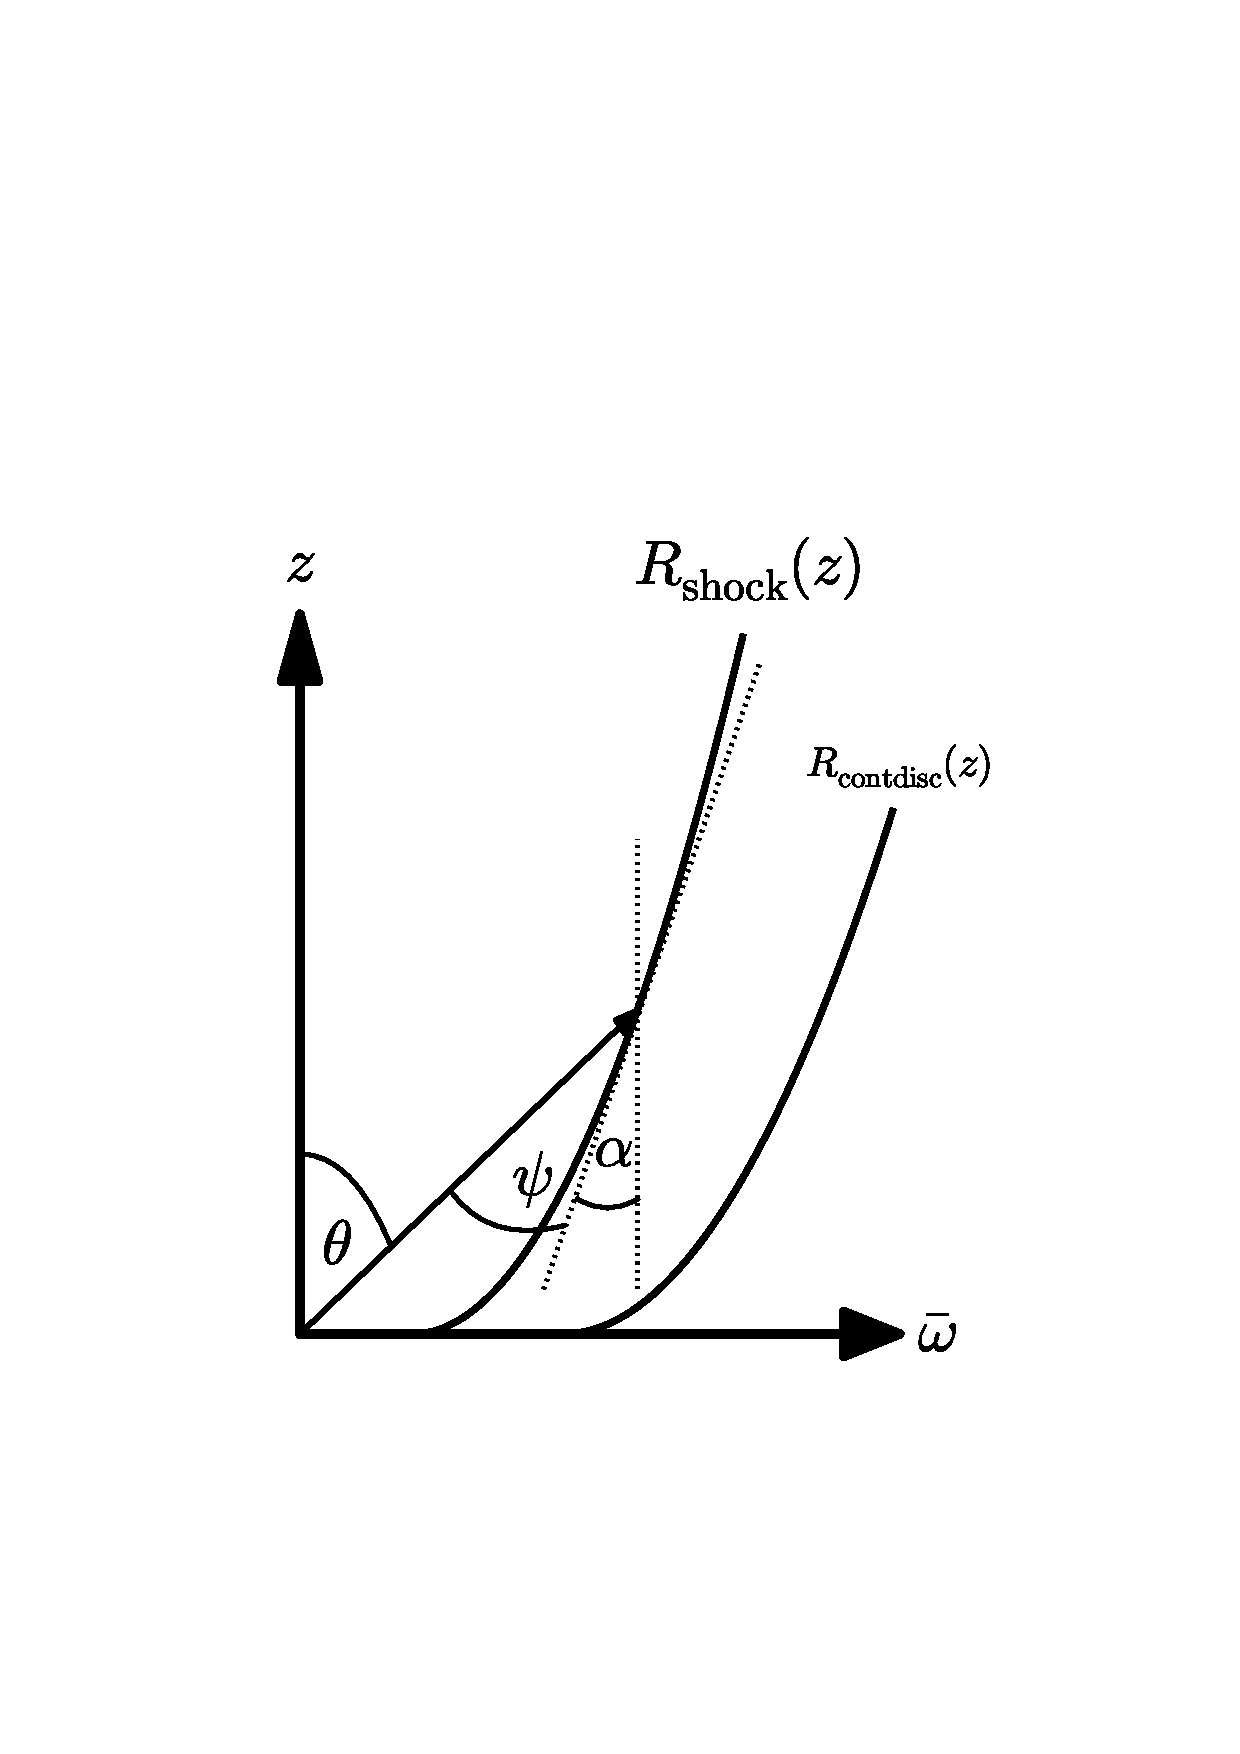
\includegraphics[width=0.35\columnwidth]{figures/sketch/sketch.png}
\caption{\label{fig:sketch}
Geometry in the $(z, \omega)$ plane. The $z$-axis is oriented along the jet, the $\omega$-axis in the plane of the circumstellar accretion disk. The innermost outflow layer is the unshocked stellar wind. The shock front is located at $R_{\rm{shock}}(z)$. The next layer is the hot, post-shock stellar wind, which is separated from the disk wind by the contact discontinuity at $R_{\rm{contdisc}}(z)$.}
\end{center}
\end{figure}

To derive the position of the shock front in the $(z, \omega)$ plane where the pre-shock ram pressure of the stellar wind and the post-shock pressure equal the external pressure $P(z)$, we need to calculate the pre-shock density $\rho_0$ and the pre-shock velocity perpendicular to the shock front $v_0$.

We assume a spherically symmetric stellar wind that is accelerated to its final velocity $v_{\infty}$ within a few stellar radii before any interaction takes place. For a given mass loss rate $\dot M$, the wind density at any distance $r$ from the central star is 
\begin{equation}\label{eqn:rho}
\rho(r) = \frac{\dot M}{4 \pi r^2 v_{\infty}}\ .
\end{equation}
Figure~\ref{fig:sketch} shows that $v_0$ depends on the position of the shock:
\begin{equation}
\label{eqn:v0}v_0 = v_{\infty} \sin \psi
\end{equation}
with 
\begin{equation}\label{eqn:angle}
\psi+\alpha =  \theta \ .
\end{equation}
Again, Figure~\ref{fig:sketch} shows how two of the angles in this equation can be calculated, so that $\psi$ can be determined. First,
\begin{equation}\label{eqn:theta}
\tan\theta = \frac{\omega}{z}\ ;
\end{equation}
second, the angle $\alpha$ is given by the derivative of the position of the shock front:
\begin{equation}\label{eqn:deriv}
\frac{\rm{d}\omega}{\rm{d}z} = \frac{\sin \alpha}{\cos \alpha} = \tan{\alpha}
\end{equation}
This gives:
\begin{equation}\label{eqn:psi}
\psi = \arctan{\frac{\omega}{z}} - \arctan{\frac{\rm{d}\omega}{\rm{d}z}}\ .
\end{equation}
Inserting equation~\ref{eqn:rho} and \ref{eqn:v0} into eqn.~\ref{eqn:Pofz}, we arrive at: 
\begin{equation}\label{eqn:P}
P(z) = \rho_0 v_0^2 = \frac{\dot{M}}{4\pi v_{\infty}(z^2+\omega^2)} v_{\infty}^2 \sin^2(\psi)
\end{equation}
Inserting eqn.~\ref{eqn:psi} this gives an ordinary differential equation (ODE), that describes the shape of the shock front:
\begin{equation}\label{eqn:ode}
\frac{\rm{d}\omega}{\rm{d}z} = \tan\left[\arctan\left(\frac{\omega}{z}\right)-\arcsin\left(\frac{\sqrt{z^2+\omega^2}}{R_0}\right)\right]
\end{equation}
with
\begin{equation}\label{eqn:r0}
R_0(z) = \sqrt{\frac{\dot{M} v_{\infty}}{4\pi P(z)}},
\end{equation}
where $R_0(z)$ is the maximal cylindrical radius of the shock front. In the case of young stars the circum-stellar disk constrains the stellar wind which cannot expand beyond the inner hole in the accretion disk at $z=0$ (Section~\ref{sect:omega0}.

The solution to the ODE determines the location of the shock front. This allows us to calculate the pre-shock velocity perpendicular to the shock front using eqn.~\ref{eqn:v0} and the post-shock temperature $T_{\mathrm{post-shock}}$. From eqn.~\ref{eqn:RH3} with negligible pre-shock pressure and $v_0=4\;v_1$ for a strong shock we derive:
\begin{equation}
T_{\mathrm{post-shock}}(z) = \frac{3}{16} \frac{\mu m_{\textrm{H}}}{k} v_0(z)^2,\label{eqn:T}
\end{equation}
where $m_{\textrm{H}}$ the mass of the hydrogen atom, $k$ the Boltzmann constant and $\mu=0.7$ is the mean particle mass for a highly ionized plasma. For general $P(z)$ the ODE needs to be solved numerically\footnote{It is possible to remove all trigonometric functions from eqn.~\ref{eqn:ode} by means of addition formulae, but that introduces singularities into the solution. Thus, we numerically solve the ODE in the form of eqn.~\ref{eqn:ode}.}. This is done in an IPython notebook \citep{PER-GRA:2007} available at \url{https://github.com/hamogu/RecollimationXrayCTTS/blob/master/scripts/jet_recol_shocks.ipynb}.


\section{Constraints on parameters}
\label{sect:parameters}
In this section we discuss observational and theoretical constraints on boundary conditions and input values for the model, most notably $P(z)$, $\dot M$, $v_\infty$, and $\omega(z=0)$. Table~\ref{tab:fiducial} shows the values we adopt for our fiducial model. We vary the parameters individually to show how each of them affects the solution of the ODE. 
\begin{table}
\label{tab:fiducial}
\caption{Values for fidcial model}
\begin{tabular}{cc}
\hline\hline
parameter & value\\
\hline
$v_\infty$ & 600 km s$^{-1}$\\
$\dot M$ & $10^{-8}\;M_\odot\textrm{yr}^{-1}$\\
$\omega_0$ & 0.01 AU\\
$P(z)$ & $P_\infty+P_0\exp\left(-\frac{z}{h}\right)$\\
$P_\infty$ & $5\cdot 10^{-6}$ Ba\\
$P_0$ & $5\cdot 10^{-4}$ Ba\\
$h$ & 2 AU\\
\hline
\end{tabular}
\end{table}

\subsection{Disk winds as boundary conditions for stellar winds}
\label{sect:boundary}
Different models exist to explain wind launching from the stellar surface \citep{1988ApJ...332L..41K,2005ApJ...632L.135M}, the X-point close to the inner disk edge \citep{1994ApJ...429..781S} and magneto-centrifugal launching from the disk \citep{1982MNRAS.199..883B,2005ApJ...630..945A}. It is likely that more than one mechanism contributes to the total outflow from the system. In this case, we expect a contact discontinuity between the different components whose position is determined by the pressure on both sides. Specifically, hydromagnetic disk winds have a tendency to collimate and possibly even to recollimate to smaller flow radii under certain conditions \citep{1982MNRAS.199..883B,1992ApJ...394..117P}.
Numerically, the magneto-centrifugally accelerated disk wind is probably the best explored component. Magneto-hydrodynamic (MHD) simulations of the disk wind have been performed in 2D \citep[e.g.][]{2005ApJ...630..945A}, 2.5D \citep[e.g.][]{2011ApJ...728L..11R} or 3D \citep[e.g.][]{2006ApJ...653L..33A}, but typically do not resolve the stellar wind, where the magneto-centrifugal launching is not effective. However, they show that the disk wind is collimated close to the axis and that the densities are largest in this region. Furthermore, the Alfv\'en surface (which separates the magnetically dominated region from the flow-dominated region) is located at many AU for the inner layers of the jet. This is in contrast with the outer, less collimated layers of the wind, which leave the magnetically dominated region at a few AUs.

\citet{2009A&A...502..217M} present analytical and numerical solutions for several scenarios that mix an inner stellar wind and an outer disk wind. In contrast to our approach, they impose a smooth transition between stellar wind and disk wind, which allows them to model the entire outflow region numerically. With some time variability in the wind launching their models produce promising knot features in the jet. In the context of our analysis, we note that the pressure in their models is magnetically dominated and much higher close to the jet axis than at larger radii in apparent contrast to Kompaneet's approximation. However, the inner jet component, that we discuss here, is so narrow that it only feels the pressure in the innermost resolution elements. The pressure at the jet axis is high in the plane of the disk and drops by one to two orders of magnitude until it reaches a plateau at $P_\infty$. Below we use a simple exponential $P(z)=P_\infty+P_0\exp\left(-\frac{z}{h}\right)$ to mimic this profile.
Similar profiles for the inner density and pressure are seen in simulations by other groups \citep[e.g.][]{2005ApJ...630..945A,Li_Krasnopolsky_Blandford_2006,2008ApJ...678.1109M}.

Observations of jets and winds from CTTS indicate that typical temperatures are a few thousand K and typical densities are in the range $10^4-10^6 \mathrm{ cm}^{-3}$ in the optically visible component \citep[e.g.][]{2000A&A...356L..41L,2007ApJ...657..897K}. This might not be the same outflow component that our model describes, but it is the best available observational estimate, so we chose the parameters of $P(z)$ to reach post-shock densities similar to these values.

Figure~\ref{fig:p_ext} shows how different pressure profiles influence the shock position. Larger pressures force the shock front onto the symmetry axes for smaller $z$ (top row). If the pressure is constant in the region where the shock front hits the symmetry axis, then the angle between the shock front and the jet axis is large, which causes high post-shock temperatures (solid red line in the upper row). In contrast, if there is a pressure gradient when the shock front bends towards the jet axis, then the shock front and the stream lines form a smaller angle and pre-shock speeds and thus the post-shock temperatures are lower (dotted black line in the top row).

The solutions shown in the bottom row of the figure are for the same pressure scale heights as those in the upper row, but here we use smaller $P_0$ for scenarios with large scale heights $h$, so that the shock front reaches the jet axis at approximately the same $z$. Close to the disk plane the pre-shock speeds differ significantly, but at large $z$ they reach very similar values. However, the scenarios with the smaller $P_0$ values reach larger radii and the slightly different shape of the shock front leads to more plasma at high temperatures.

\begin{figure}[h!]
\begin{center}
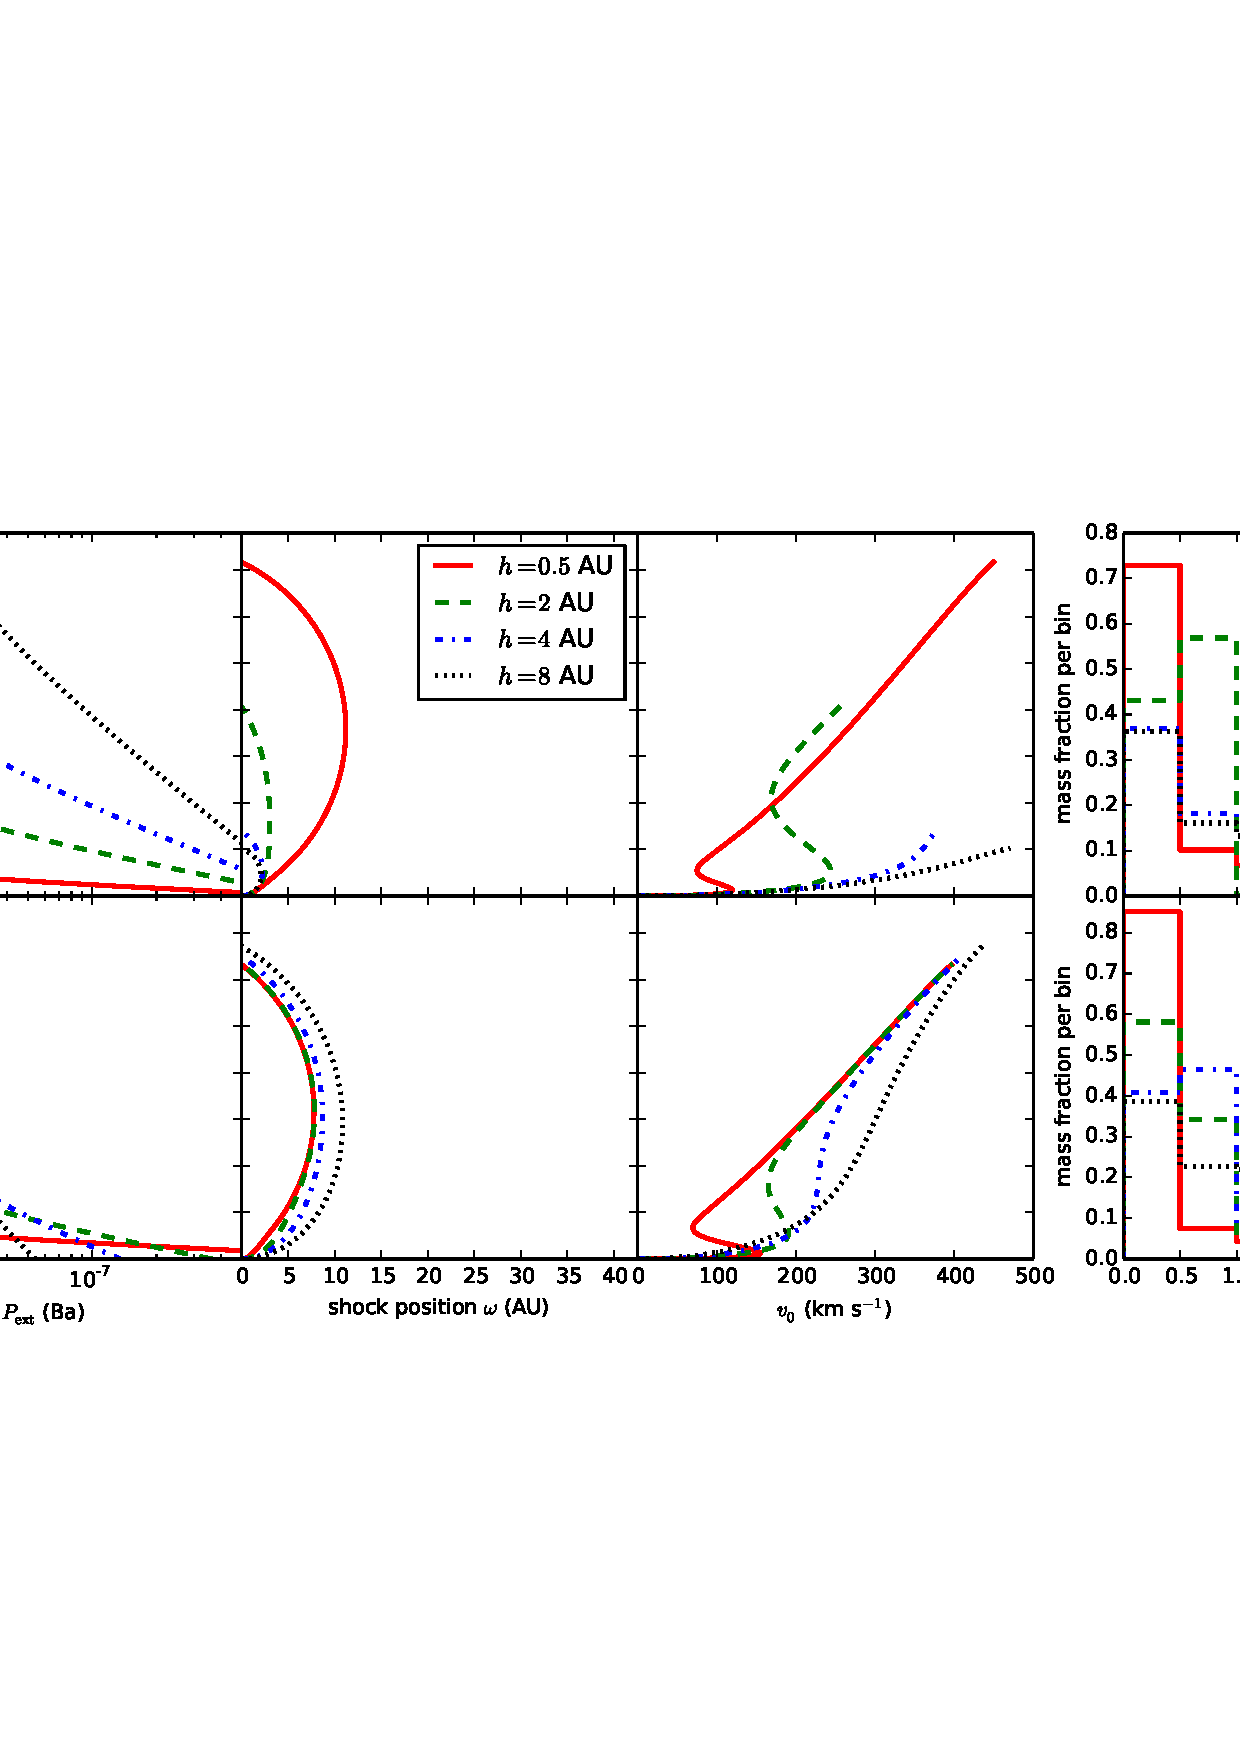
\includegraphics[width=1\columnwidth]{figures/P_ext/P_ext.png}
\caption{\label{fig:p_ext}
Solutions to the ODE for different exponential pressure profiles. In the top row the scale height $h$ of the exponential is varied with all other parameters held fixed; the bottom row uses the same values for $h$, but also scales $P_0\propto h^{-1.5}$.
The four panels show imporant variables for each solution. 
\emph{leftmost panel}: Profile of the external pressure $P(z)$. 
\emph{middle left panel}: Position of the shock front. Note that the two axes in this panel are to scale. The unshocked stellar wind region is much longer in $z$ direction (height above the disk) than it is wide. 
\emph{middle right panel}: Pre-shock velocity $v_0$ measured perperdicular to the shock front. 
\emph{rightmost panel}: Distribution of post-shock temperatures, weighted by spherically integrated mass flux. This distribution is dominated by the temperature (which in turn is set by $v_0$) at small values of $z$, since the shock surface is close to the central object and covers a large solid angle of the stellar wind and therefore a large fraction of the total mass flux. Note that this panel does not show an emission measure distribution of all observed plasma; it only shows which fraction of the mass is heated to what temperature in the shock. It does not account for the fact that this plasma will eventually cool and contribute emission at cooler temperatures; a simulation of the thermodynamics of the cooling plasma is beyond the scope of this article.}
\end{center}
\end{figure}

\subsection{Mass-loss rates}
The measured mass loss rates in the outflows from CTTS vary widely between objects.  Even for a single object, very different mass loss rates can be found, depending on the spectral tracers chosen and on the assumptions used to calculate mass loss rates from line fluxes. The filling factor that describes the fraction of the observed volume occupied by hot gas is especially uncertain because the innermost jet component is generally not resolved.

Typical mass loss rates found in the literature for CTTS outflows are in the range $10^{-10}-10^{-6}M_{\odot}\textrm{ yr}^{-1}$ \citep{1999A&A...342..717B,2006A&A...456..189P}. For example, \citet{2006ApJ...646..319E} measure values down to $10^{-10}$~M$_{\odot}$~yr$^{-1}$ for some CTTS, but only upper limits for weak-line T Tauri stars (or WTTS). In the specific case of DG~Tau \citet{1997A&A...327..671L} calculate the  mass loss rate as $6.5\cdot 10^{-6}$~M$_{\odot}$~yr$^{-1}$; \citet{1995ApJ...452..736H}
obtain $3\cdot 10^{-7}$~M$_{\odot}$~yr$^{-1}$ and, further out in the jet, \citet{2000A&A...356L..41L} find $1.4\cdot 10^{-8}$~M$_{\odot}$~yr$^{-1}$. Those measurements for the optical jet are probably dominated by the disk wind \citep[e.g.][]{2014arXiv1404.0728W} and unlikely to track the stellar mass loss correctly.
Paper~I shows that a mass loss below $10^{-10}$~M$_{\odot}$~yr$^{-1}$ is sufficient to explain the X-ray emission from the jet as shock heating.
We use $10^{-8}$~M$_{\odot}$~yr$^{-1}$ as fiducial stellar mass loss in the remainder of the article. This is only a fraction to the total mass loss of the system and the disk wind, though slower, operates over a much larger area dominates the system's mass loss in our scenario.

Figure~\ref{fig:dot_m} shows how a larger mass loss rate and therefore a higher density and ram pressure in the stellar wind pushes the shock front out to larger radii and heights. The different shape of the shock front also influences the post-shock temperatures. In the high mass loss rate scenario (black dotted line) the shock front reaches its maximum radius at 60~AU and most of the spherically symmetric wind passes the shock front at shallow angles, so this scenario has the highest fraction of low temperature material.


\begin{figure}[h!]
\begin{center}
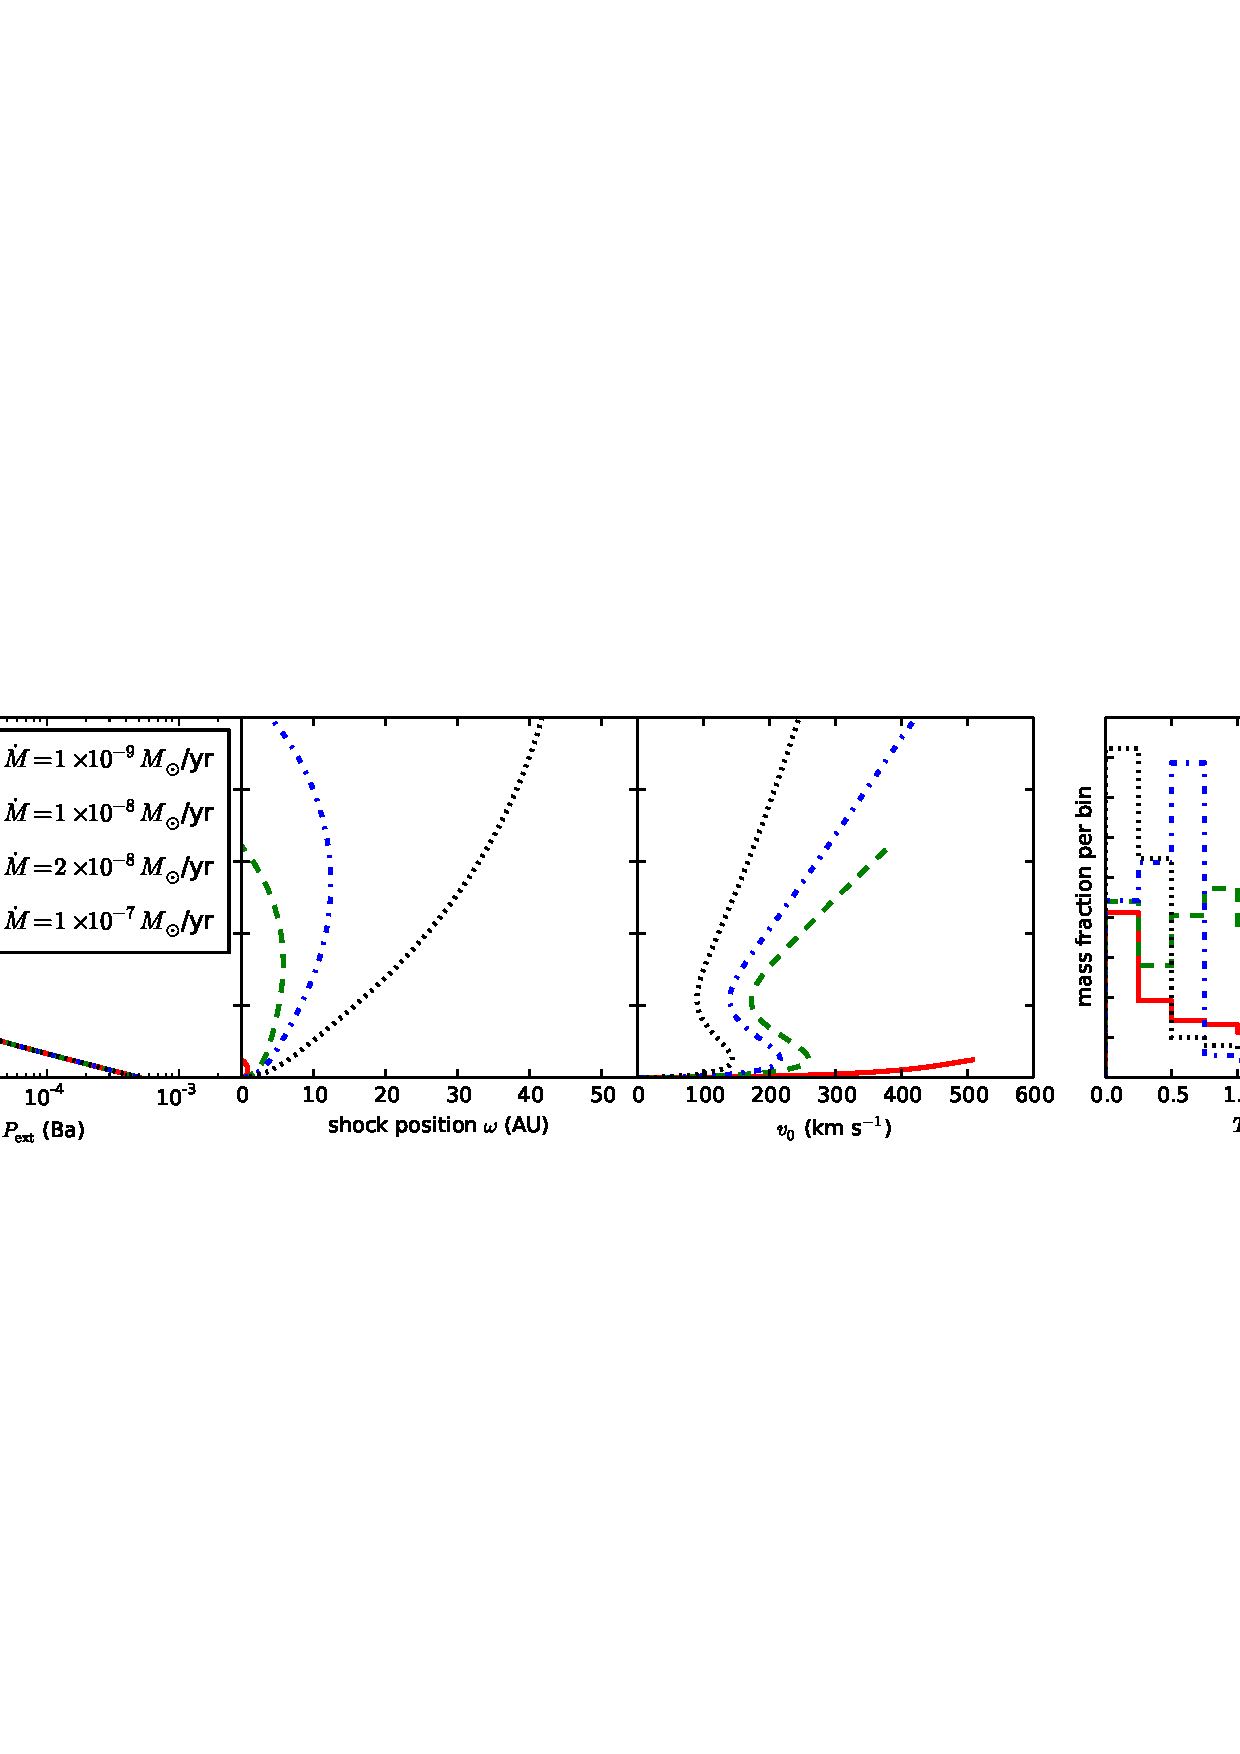
\includegraphics[width=1\columnwidth]{figures/dot_m/dot_m.png}
\caption{\label{fig:dot_m}
Solutions to the ODE for different mass loss rates. For a description of the individual panels see Fig.~\ref{fig:p_ext}. The middle left panel only shows the region close to the star for clarity. The shock front with the largest mass loss rate extends to $\omega=40$~AU and comes back to the axis of symmetry at 130~AU.}
\end{center}
\end{figure}

\subsection{Wind speed}
The launching mechanism of the stellar wind in CTTS is uncertain. \citet{2007IAUS..243..299M} show that stellar winds from CTTS cannot have a total mass loss above $10^{-11}M_\odot\mathrm{ yr}^{-1}$ if they are launched hot. Otherwise, the high densities required to reach such a mass loss would lead to a runaway cooling. 
This would probably hinder the wind  launching and should be also observable. Thus, the winds of CTTS are probably more complex than just a scaled up version of the solar wind. Still, the wind speeds observed in the sun provide a reasonable estimate for $v_\infty$. The solar wind consists of a slow wind with a typical velocity of 400~km~s$^{-1}$ and a fast wind around 750~km~s$^{-1}$ \citep{2005JGRA..110.7109F}. The relative contribution and the launching position of the two types changes over the solar cycle, but the slow wind often emerges from regions near the solar equator and fast wind is generally associated with coronal holes \citep{1999GeoRL..26.2901G,2003A&A...408.1165B,2009LRSP....6....3C}. Despite these differences, the total energy flux in the solar wind is almost independent of the latitude, because the slower wind is denser than the faster wind \citep{2012SoPh..279..197L}. In this article, we set $v_\infty=600$~km~s$^{-1}$ as the fiducial outflow velocity and we assume that the wind is accelerated close to the star and has reached $v_\infty$ before it interacts with the shock front. We use a spherically symmetric stellar wind with a constant velocity. For a solar-type wind this works well for deriving the shape of the shock front because eqn.~\ref{eqn:r0} depends only on the total energy flux $\rho v^2_\infty \propto \dot M v_\infty$ and not the velocity itself. 

Figure~\ref{fig:v_infty} shows how a large $v_\infty$ and a correspondingly large ram pressure of the stellar wind push the shock front higher above the disk plane, similar to outflows with a larger $\dot M$. Additionally, $v_\infty$ is the single most important parameter that controls the maximal post-shock temperatures and the amount of hot plasma.
The figure shows that high shock speeds and thus high post-shock velocities are reached close to the disk plane. Because this region covers a large solid angle, it is an important contributor to the total temperature distribution of the post-shock plasma (rightmost panel). However, the temperature in this region is probably overestimated by our model because the wind may not have reached $v_\infty$ this close to the star or the wind may not be spherically symmetric. A lower wind velocity and higher density at the equator would lead to lower post-shock temperatures with a higher emission measure close to the disk plane.


\begin{figure}[h!]
\begin{center}
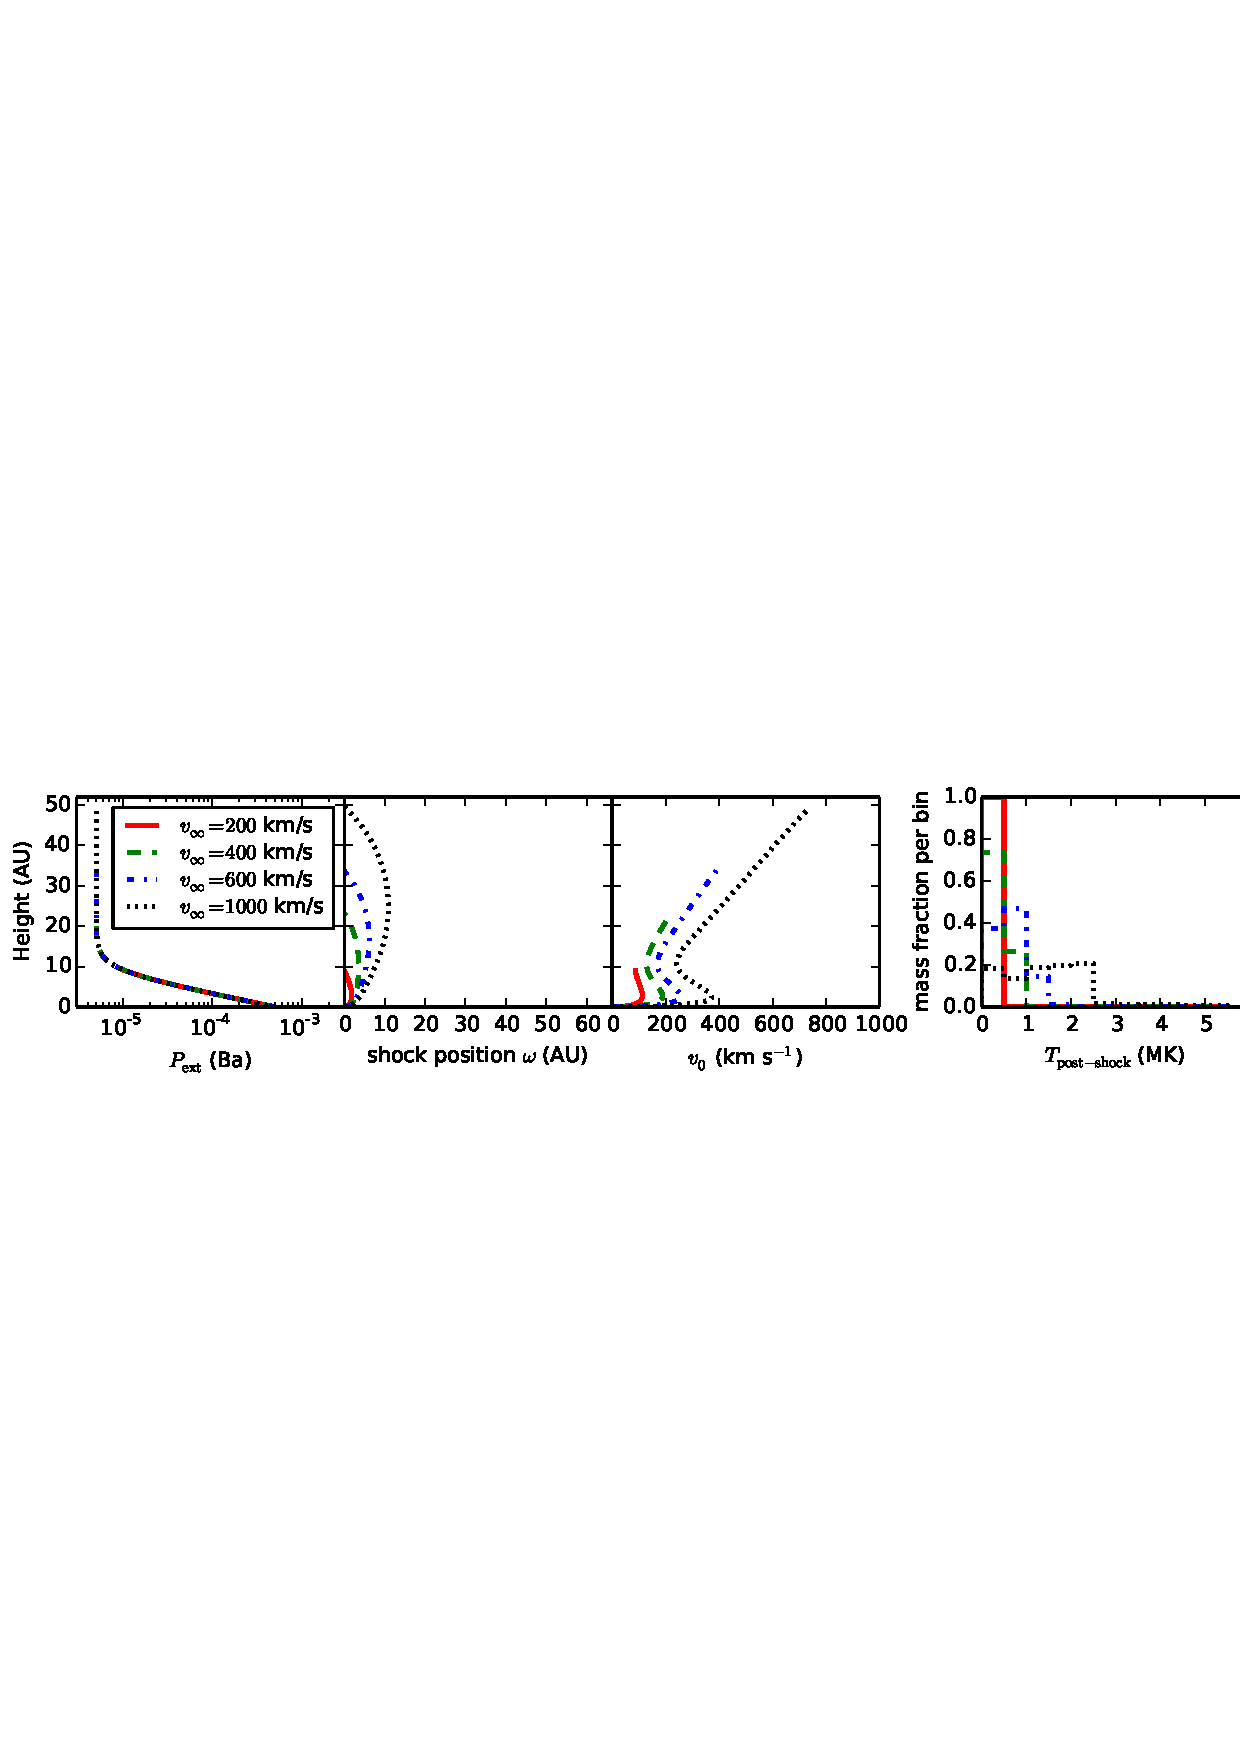
\includegraphics[width=1\columnwidth]{figures/v_infty/v_infty.png}
\caption{\label{fig:v_infty}
Solutions to the ODE for different $v_\infty$. For a description of the individual panels see Fig.~\ref{fig:p_ext}.}
\end{center}
\end{figure}

\subsection{Starting point of integration}
\label{sect:omega0}
From a mathematical point of view, the starting point of the integration in the plane of the disk can be chosen freely anywhere between $\omega=0$ and $\omega=R_0(z=0)$. Figure~\ref{fig:omega_0} compares different starting points under otherwise equal conditions. For small initial radii the ram pressure of the stellar wind pushes the shock surface out to larger radii in a comparatively small $\Delta z$. This leads to small pre-shock speeds in this region because the direction of the flow and the shock surface are almost parallel. This region also represents a large fraction of the total mass loss of the stellar wind, because it covers a large angle in the $(z,\omega)$-plane and a large solid angle of the spherical wind emission. Consequently, models with small values for $\omega_0$ show much less material that is heated up to high temperatures. 

Physically, the position of the shock front is restricted by the position of the disk - the shock between the stellar wind and the disk material (in the disk itself or the disk wind) must occur within the inner hole of the disk. Fortunately, figure~\ref{fig:omega_0} shows that the two solutions for $\omega_0=0.01$~AU and $0.1$~AU are almost indistinguishable and the exact value for this parameter is not important as long as it is small. We use $\omega_0 = 0.01$~AU as the fiducial starting point for the integration.

\begin{figure}[h!]
\begin{center}
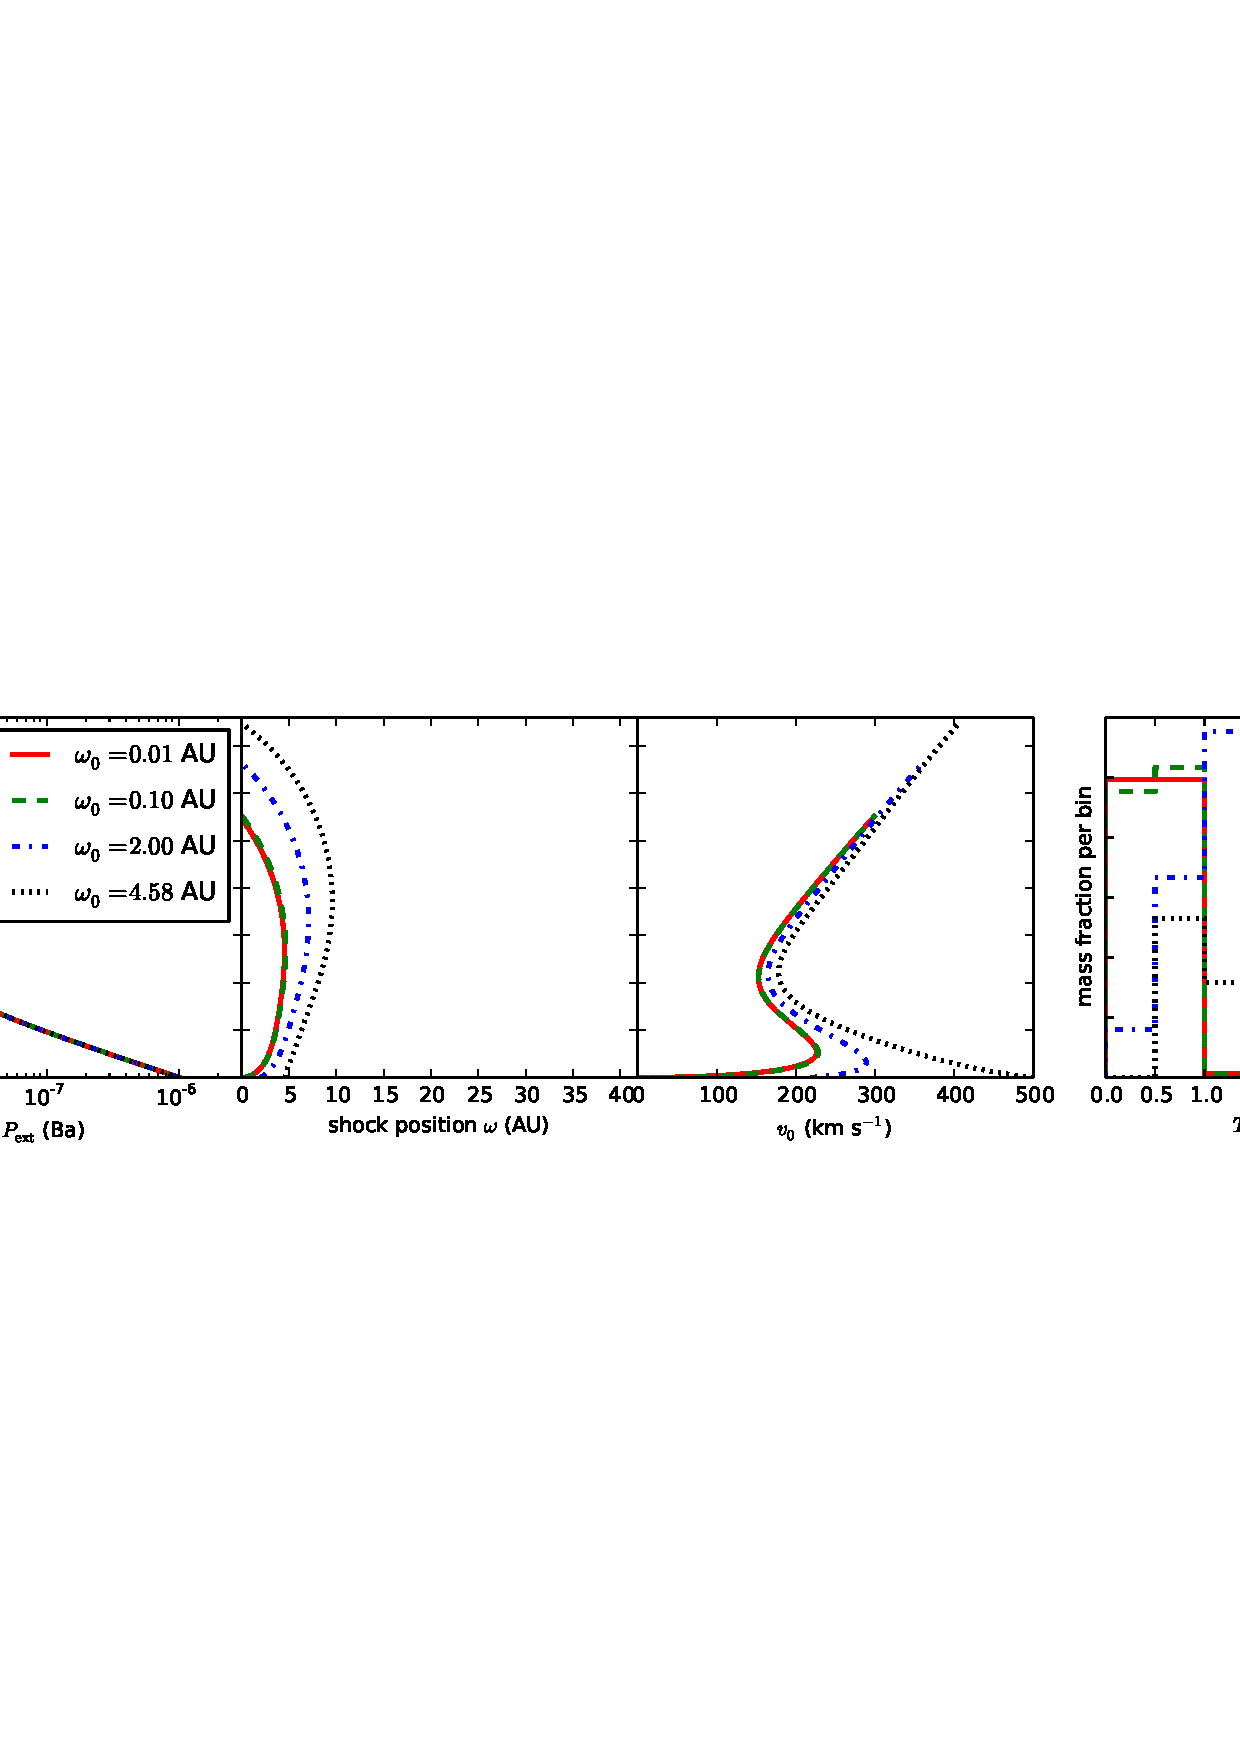
\includegraphics[width=1\columnwidth]{figures/omega_0/omega_0.png}
\caption{\label{fig:omega_0}
Four solutions to the ODE for four different starting points $\omega(z=0)=\omega_0$. For a description of the individual panels see Fig.~\ref{fig:p_ext}.}
\end{center}
\end{figure}

\subsection{Initial wind temperature}
\label{sect:T_0}
In Section~\ref{sect:model} we developed our model for an initially cold stellar wind where the thermal presure before the shock can be ignored. This is motivated by two arguments: (i) \citet{2007IAUS..243..299M} show that hot stellar winds will cool quickly and cause X-ray emission much brighter than observed if they have a mass loss rate above $10^{-11}M_\odot\mathrm{ yr}^{-1}$. Since we need mass loss rates well above this value to explain the resolved X-ray emission at 40~AU, the wind must be launched cold. (ii) The solar wind has 1~MK. It is unclear which physical process heats it to this temperature, but it is probably related to magnetic waves. In CTTS the wind mass loss rate is higher than in the Sun, and it seems unlikly that the same mechanim can provide enough energy to heat a stellar CTTS wind to the same temperature.

The approximation to neglect the initial wind temperature is valid to a few $10^5$~K for the densities and wind speeds considered here. Hotter winds cannot be described in our model, because their sound speed is so large that no strong shock develops for small angles $\psi$.

\section{Results}
\label{sect:results}
The last section already showed that for all parameters consistent with the theoretical and observational constraints the stellar wind is enclosed in a finite region by a shock front. This shock front generally reaches a maximum cylindrical radius of only several AUs, but a much larger height above the accretion disk for external pressure profiles with high pressure in the plane of the disk and a large pressure gradient (fiducial model in Fig.~\ref{fig:result}). A shallower pressure profile leads to a stellar wind region that is wider.So far, no stellar wind zone is resolved within the more massive and wider disk wind in any CTTS imaging, limiting the maximal size of the stellar wind region to a few AU. Our calculations show that this scenario is compatible with the known properties of the stellar wind. The biggest uncertainty is probably the value of the external pressure. As discussed above, different simulations in the literature predict similar pressure profiles, but the normalization of the pressure depends to a large degree on the disk magnetic field, which is only poorly constrained. In our calculation, we have scaled the pressure such that the post-shock densities are compatible with observations of the jet and we find a fiducial model that is compatible with the X-ray emission from the jet that we set out to explain. However, the magnitude of the pressure is a free parameter in our model and if it could be determined more accurately, that will confirm or rule-out the scenario we suggest in this article.

The highest post-shock temperatures are generally reached at the base of the jet when the stellar wind encounters the inner disk rim or at large $z$ when the shock front intersects the jet axis. Thus, the position of the hottest post-shock cooling plasma must be very close to the jet axis. In our fiducial model (Fig.~\ref{fig:result}, solid red line), the temperature is just sufficient to produce X-ray emission. Paper~I showed that in DG~Tau a small faction, about $10^{-3}$, of the total mass loss rate in the outflow is enough to power the observed X-ray emission at the base of the jet. Figure~\ref{fig:rhocool} shows the pre-shock number densities $n_0$ for the four models from Fig.~\ref{fig:result}. A detailed treatment of the post-shock region is beyond the scope of this paper, but an upper limit on the post-shock cooling length $d_{\mathrm{cool}}$ can be derived according to \citet{2002ApJ...576L.149R}:
\begin{equation}
d_{\mathrm{cool}} \approx 20.9 \mathrm{ AU}
    \left(\frac{10^5\mathrm{ cm}^{-3}}{n_0}\right)
    \left(\frac{v_{\mathrm{shock}}}{500\mathrm{ km s}^{-1}}\right)^{4.5}\ .
\end{equation}
The derivation for this formula assumes a cylindrical cooling flow. In contrast, in our model the external pressure will continue to compress the gas, as it starts cooling. Since denser gas emits more radiation and thus cools faster, $d_{\mathrm{cool}}$ is only an upper limit. With this in mind, figure~\ref{fig:rhocool} (lower panel) indicates that the cooling lengths for our fiducial model is consistent with the X-ray observations that do not resolve the wind shock \citep{2008A&A...488L..13S}. Since only a very small fraction of the stellar mass loss is heated to X-ray emitting temperatures (Fig.~\ref{fig:result}, rightmost panel) the low-mass loss scenario also does not provide enough X-ray luminosity to explain the observations (paper~I).
Significantly higher pressures require unrealistically fast outflows to push the shock front out to 40~AU and lower pressures do not allow a mass flux high enough to power the X-ray luminosity.

In our model, it is irrelevant how much of the external pressure is provided by the magnetic field in the disk wind and how much by thermodynamic pressure. The region of interest is still within the Alfv\'en surface (see references in Sect.~\ref{sect:boundary}), so the influence of the magnetic field probably dominates. Otherwise, the disk wind would also have to be very dense (probably too dense to be consistent with observations) to provide this pressure. Observationally, it is difficult to distinguish the stellar wind from the disk wind. The slower jet components observed further away from the jet axis carry much of the mass flow \citep{2000ApJ...537L..49B}. Their origin is probably the inner region of the disk and not the star \citep{2003ApJ...590L.107A}. Thus, it is fully consistent that our model predicts a mass loss fraction larger than  $10^{-3}$ of the stellar wind at X-ray emitting temperatures. If the disk wind dominates over the stellar wind in mass loss, then the fraction of hot gas in the (stellar plus inner disk) jet might still be small.

\begin{figure}[h!]
\begin{center}
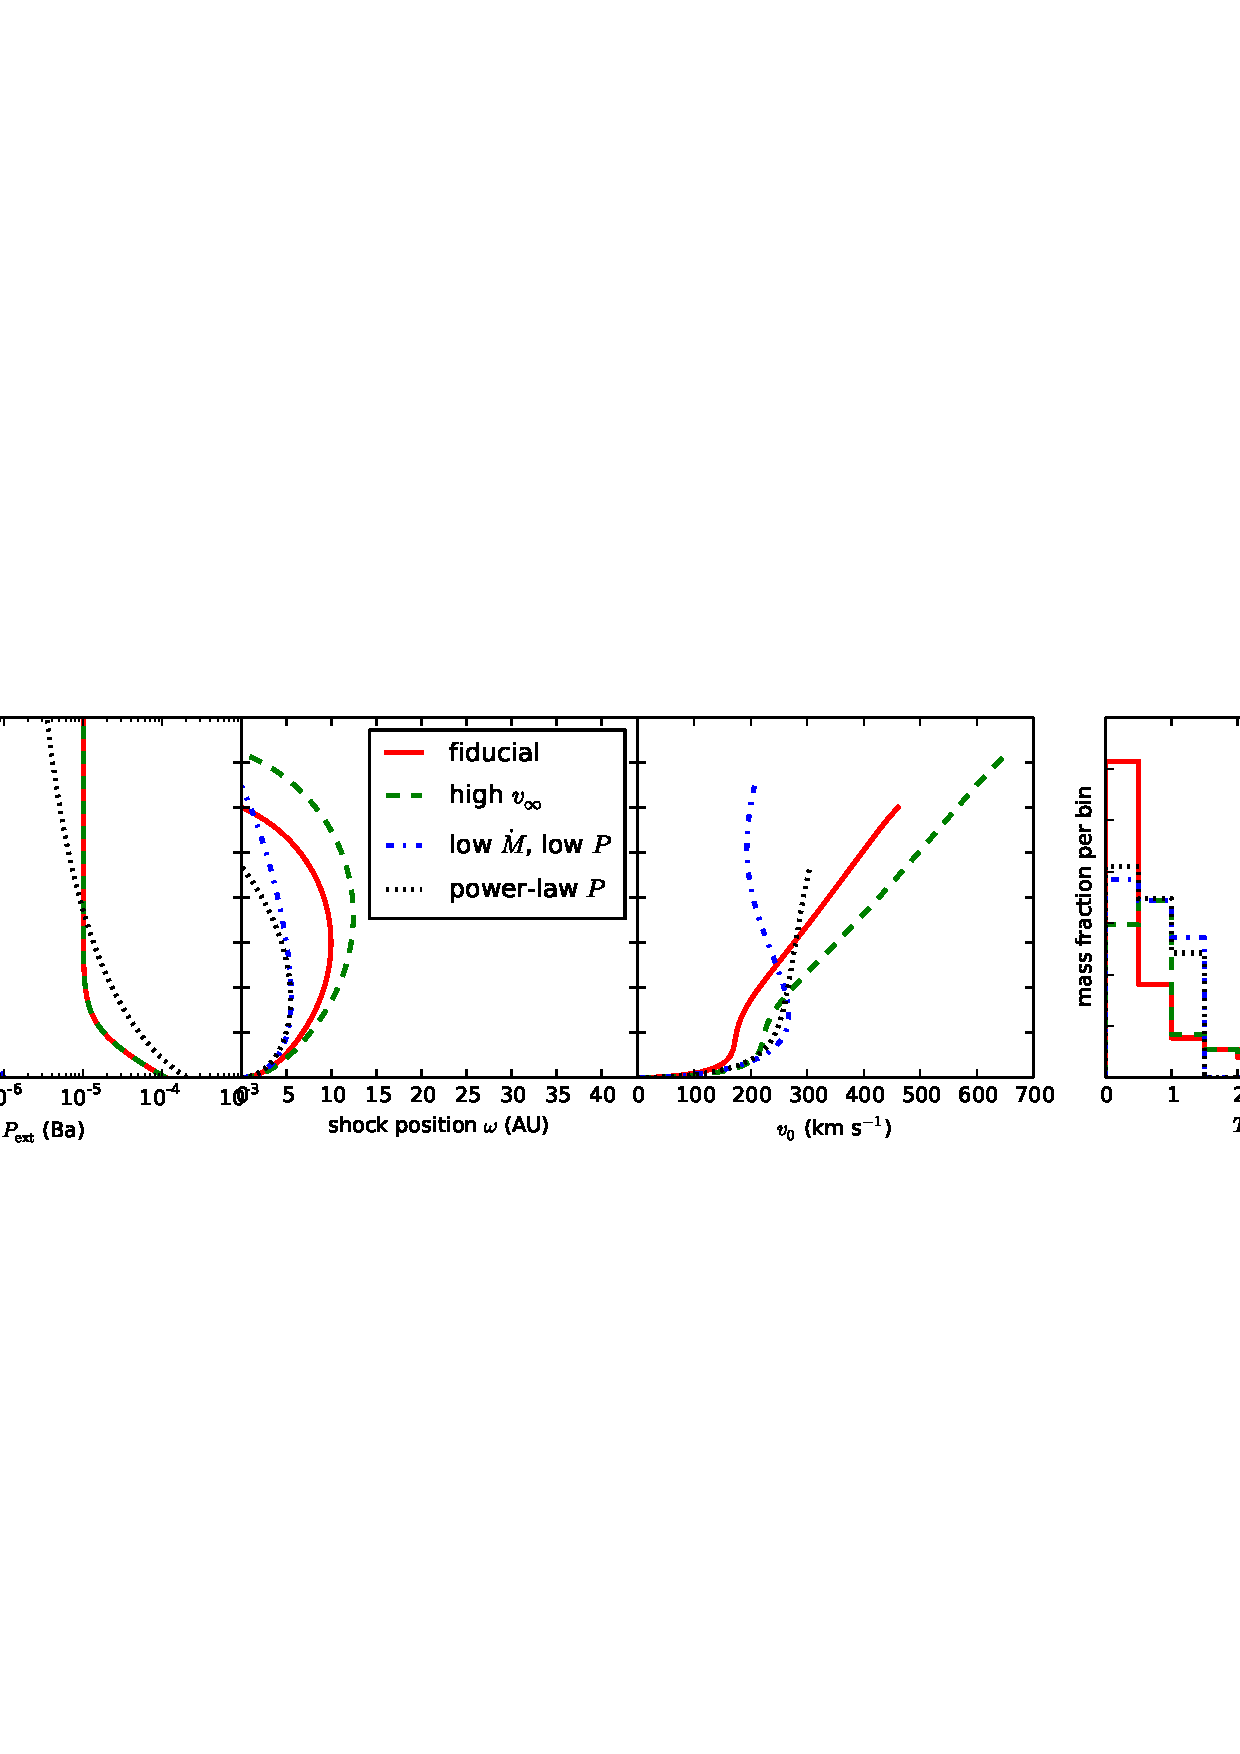
\includegraphics[width=1\columnwidth]{figures/result/result.png}
\caption{\label{fig:result}
Different scenerios with parameters well withing the range observed for CTTS predict a stellar wind shock that reaches 20-40~AU along the jet, but extends only few AU in the radial direction. For a description of the individual panels see Fig.~\ref{fig:p_ext}.}
\end{center}
\end{figure}

\begin{figure}[h!]
\begin{center}
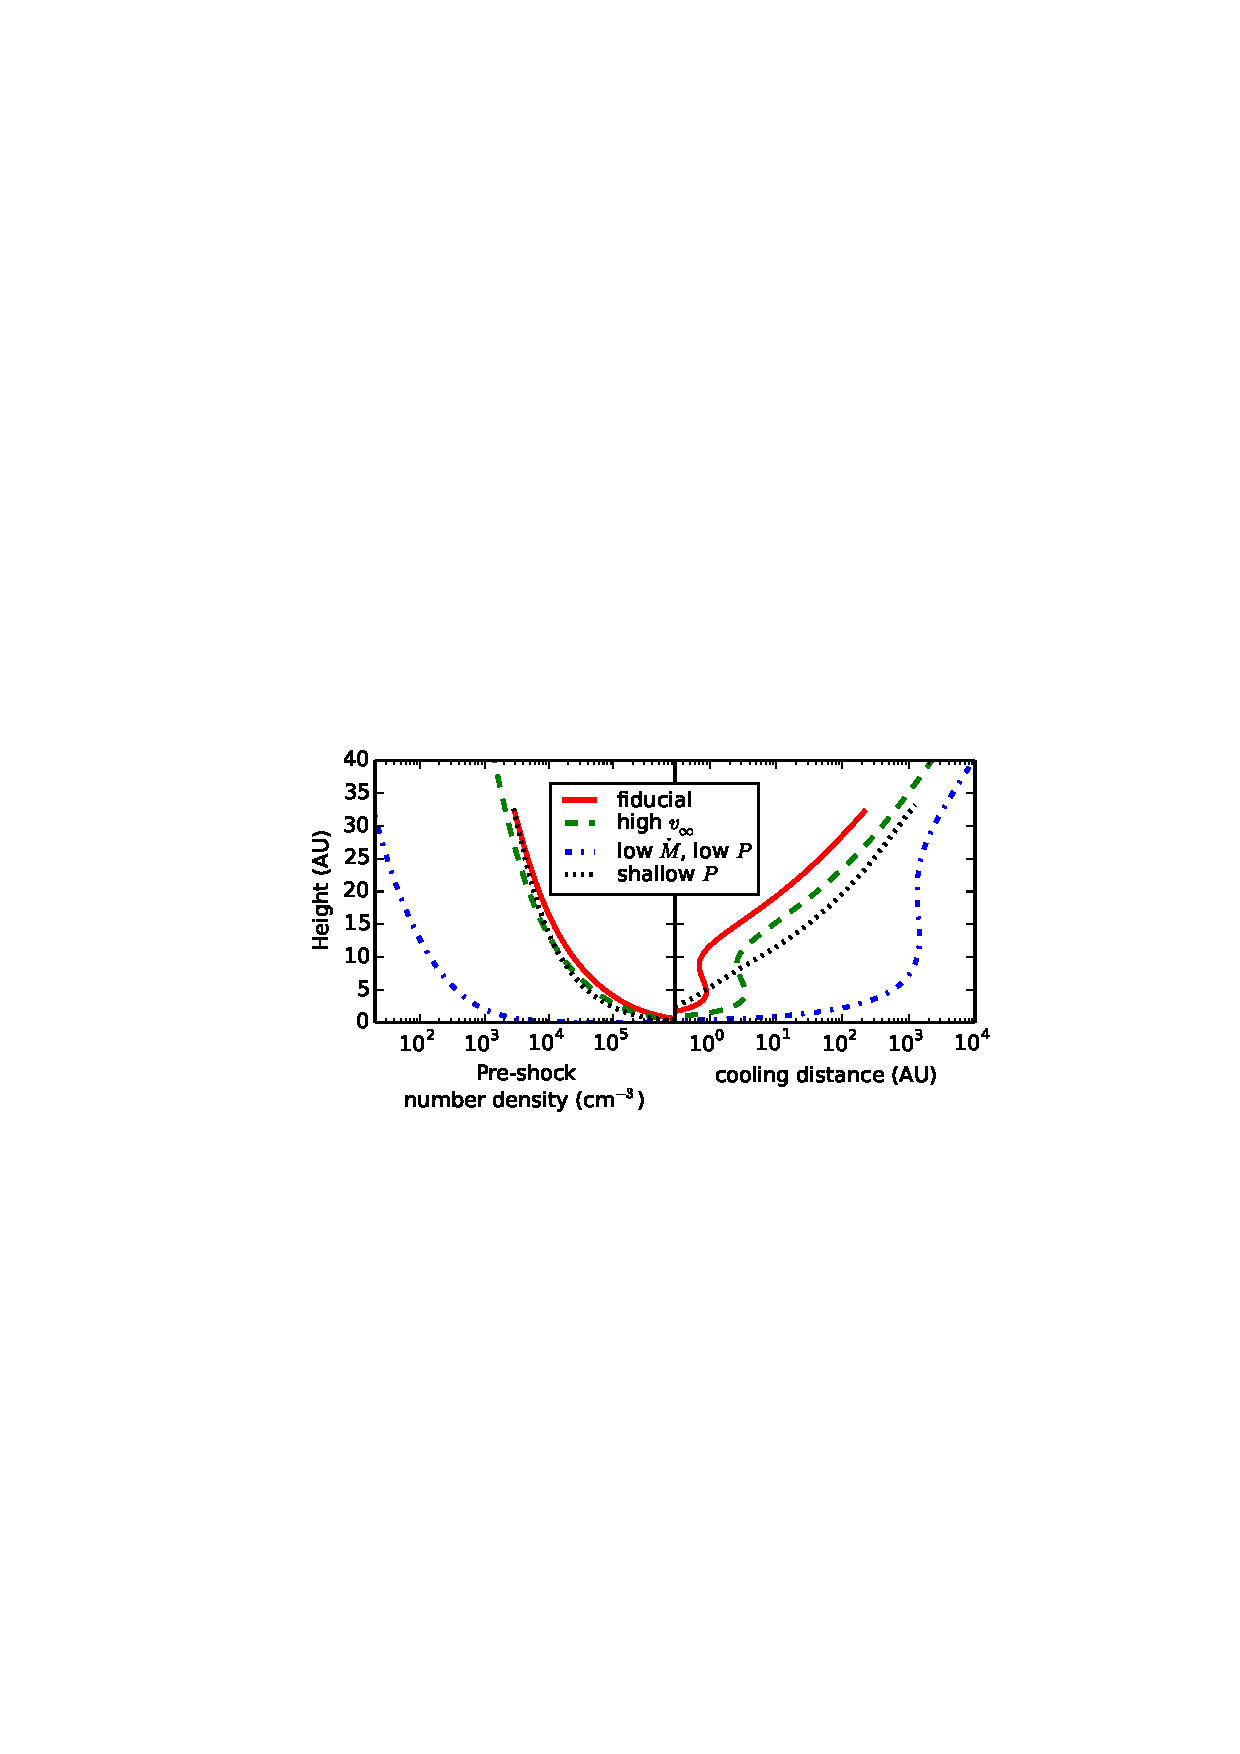
\includegraphics[width=0.42\columnwidth]{figures/rhocool/rhocool.png}
\caption{\label{fig:rhocool}
Post-shock number density and an estimate (see text) of the cooling distance for the shock models shown in Fig.~\ref{fig:result}.}
\end{center}
\end{figure}

\section{Discussion}
\label{sect:discussion}
In a CTTS system, stellar wind and disk wind interact. The high pressure of the disk wind can confine the stellar wind into a narrow, jet-like region, bound by an elongated shock surface. For reasonable parameters of $\dot M$, $v_\infty$, $\omega_0$ and $P(z)$ the shock surface encloses a region only several AU wide but tens of AU along the jet axis. 
 
The shock surface is so small that it cannot be resolved with current instrumentation and therefore cannot be seen directly as a cavity in the disk wind. A small fraction of the stellar wind is shocked to X-ray emitting temperatures $>1$~MK and provides a stationary X-ray source consistent with observations. 
Paper~I showed that a shock with these properties is required to explain the observed X-ray emission in the CTTS DG~Tau if shocks are major heating agents. We show that such a shock naturally arises in a scenario where the stellar wind is confined by an external pressure and feeds the innermost layers of the jet.
Furthermore, \citet{2013A&A...550L...1S} observed C\;{\sc iv} emission in DG Tau that is formed at cooler temperatures than those required for X-ray emission and that is too luminous to be explained by cooled X-ray plasma alone. Almost all solutions of the ODE describing the interaction of stellar and disk wind have more plasma heated to 0.5~MK than to 1~MK and can in principle explain these observations as well. In recent observations in the IR \citet{2014arXiv1404.0728W} also identified a stationary emission region on the jet axis about 40~AU from the central star. They interpret the X-rays,  C\;{\sc iv}, and their own [ Fe\;{\sc ii}] data all as a signature of the same shocked jet, while \citet{2013A&A...550L...1S} point out that the C\;{\sc iv} luminosity is too large to be powered by just the cooling X-ray plasma. Looking at the post-shock temperature distribution in Fig.~\ref{fig:result}, our model can naturally explain how multiple temperature components arise in the stellar wind.

However, more detailed numerical simulations of the post-shock cooling zone and the shape of the contact discontinuity between the disk wind and the post-shock stellar wind are required to check whether the physical extent of the cooling region behind the shock front and the position of the peak  C\;{\sc iv} emission can be matched to the observations.

\citetp{1993ApJ...409..748G} discussed a similar idea as we do here, where they aim to explain the forbidden optical emission lines seen from CTTS with a shock due to the recollimation of the jet outflow. In contrast to our model, they attribute it to the shocked disk wind, not the stellar wind. At the time, the high-temperature emission from CTTS jets was not known and that seems to be a natural choice to keep the shock velocity low. However, a shocked disk wind cannot supply the high shock velocities to explain the resolved X-ray and \ion{C}{4} emission that we now see. On the other hand, it is possible that our model, a shocked stellar wind, will also produce some fraction of the optical line emission.
Remember that our stellar wind is collimated because it is embedded into a strong disk wind, so we expect that the low-temperature emission from the stellar wind is small compared to the low-temperature emission from the surrounding disk wind. Only for high temperatures (X-ray and FUV emission), the stellar wind will dominate and our model provides a mechanism to explain this emission with a stationary shock front, while disk wind models often require unrealistically high launching velocities to reach X-ray emitting temperatures in oblique shocks. The price we pay is the requirement for stellar mass loss rates orders of magnitude above those of main-sequence stars.

There is too much parameter degeneracy to turn the argument around and derive $\dot M$ and  $v_\infty$ from the fact that we observe X-ray and FUV emission a few tens of AUs from the star, but our models requires a certain range of external pressures $P(z)$. Too high pressures push the shock front back to the jet axis very close to the star and too low pressures cannot confine the shock region within a few tens of AU.



\section{Summary}
\label{sect:summary}
A fast stellar wind that is confined by an external pressure from the disk wind will form a stationary collimation shock. We derive the geometrical shape and other properties of this shock front and find that this model provides a viable explanation of the soft X-ray and FUV emission observed at the base of young stellar jets, specifically in DG~Tau.

Acknowledgement: Support for this work was provided for HMG by NASA through grant GO-12907.01-A from the Space Telescope Science Institute, which is operated by the Association of Universities for Research in Astronomy, Inc., under NASA contract NAS 5-26555 and by NSF AST1313083 and NASA NNX14AB38G for ZYL.

\bibliography{bibliography/converted_to_latex.bib}

\end{document}

